\documentclass[border=2pt]{standalone}
\usepackage[T1]{fontenc}\usepackage{mathptmx}
\usepackage{amsmath,amssymb}\usepackage{tikz}\usepackage{pgfplots}
\pgfplotsset{compat=1.18}
\usetikzlibrary{shapes.geometric, arrows.meta, positioning, calc}
\setlength{\columnwidth}{3.45in}
\newcommand{\Pfree}{P_{\mathrm{free}}}\newcommand{\dfree}{d_{\mathrm{free}}}\newcommand{\pos}{\mathrm{pos}}
\newcommand{\ind}{\mathbf{1}}\newcommand{\Lin}{\mathcal{L}}
\pgfplotsset{ieeeplot/.style={width=\columnwidth, height=5.4cm,
 tick label style={font=\footnotesize}, label style={font=\footnotesize},
 legend style={font=\footnotesize, draw=black!60, fill=white, fill opacity=0.9, text opacity=1},
 grid=both, grid style={line width=0.2pt, draw=black!15}, major grid style={line width=0.3pt, draw=black!25},
 every axis plot/.append style={line width=0.8pt, mark size=2.2pt}}}
\begin{document}
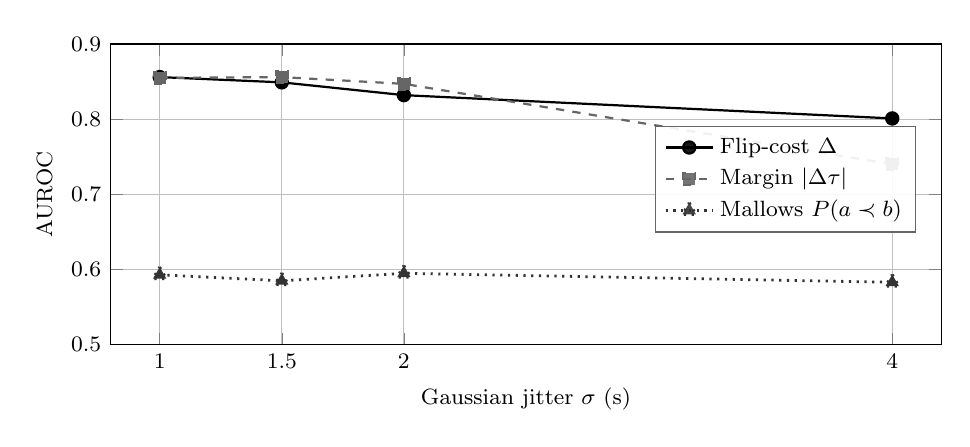
\begin{tikzpicture}
\begin{axis}[ieeeplot,
  xlabel={Gaussian jitter $\sigma$ (s)}, ylabel={AUROC},
  xmin=0.8, xmax=4.2, ymin=0.5, ymax=0.9,
  xtick={1,1.5,2,4}, ytick={0.5,0.6,0.7,0.8,0.9},
  legend style={at={(0.97,0.55)}, anchor=east}, legend cell align=left]
\addplot[black, solid, mark=*] coordinates {(1.0,0.856) (1.5,0.849) (2.0,0.832) (4.0,0.801)};
\addlegendentry{Flip-cost $\Delta$}
\addplot[black!60, dashed, mark=square*] coordinates {(1.0,0.855) (1.5,0.856) (2.0,0.847) (4.0,0.740)};
\addlegendentry{Margin $|\Delta\tau|$}
\addplot[black!80, dotted, mark=triangle*, mark size=2.8pt, line width=1pt] coordinates {(1.0,0.593) (1.5,0.585) (2.0,0.595) (4.0,0.583)};
\addlegendentry{Mallows $P(a\prec b)$}
\end{axis}
\end{tikzpicture}
\end{document}
